\documentclass[tikz]{standalone}

\definecolor{mLightGreen}{HTML}{14B03D}

\begin{document}

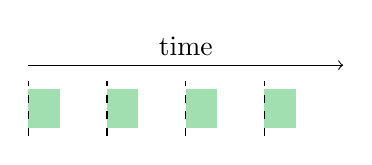
\begin{tikzpicture}
\draw[->] (0, 0.8) -- node[above] {time} (4, 0.8);

\fill [mLightGreen,opacity=0.4] (0, 0) rectangle (0.4, 0.5);
\draw[dashed] (0, -0.1) -- (0, 0.6);

\fill [mLightGreen,opacity=0.4] (1, 0) rectangle (1.4, 0.5);
\draw[dashed] (1, -0.1) -- (1, 0.6);

\fill [mLightGreen,opacity=0.4] (2, 0) rectangle (2.4, 0.5);
\draw[dashed] (2, -0.1) -- (2, 0.6);

\fill [mLightGreen,opacity=0.4] (3, 0) rectangle (3.4, 0.5);
\draw[dashed] (3, -0.1) -- (3, 0.6);

\end{tikzpicture}

\end{document}